\section{eBPF}
  \subsection{Berkeley Packet Filter}
    StevenとVan \cite{mccanne1993bsd}は1993年に,Unix系のOS上でパケットキャプチャを効率的に行うためのアーキテクチャである
    BSD Packet Filterを提案した.以下,Berkeley Packet Filterを「BPF」と表記する. \\
    論文発表当時のパケットキャプチャでは,カーネル空間で取得したパケットをすべてユーザー空間にコピーしてからフィルタリングしていて,
    これが無駄なオーバーヘッドの原因となっていた.
    \cite{mccanne1993bsd}は特殊な32ビット命令で記述されたプログラムを解釈して
    フィルタリングを行う疑似マシン (BPF pseudo-machine) を考案し,それをカーネル空間で動作させることでこの問題に対処した.
    既存のシステムとの比較では,BPFは最大で20倍程度高速に動作した.
    BPFのアーキテクチャの概要を\Fref{img:bpf_old}に示す.
    
    BPFはLinuxカーネルのv2.1.75にてLinux Socket Filterという名前で導入され,\texttt{tcpdump}コマンドの高速化のために使われた.
    
  \subsection{BPFの拡張}
    BPFはLinuxカーネルのv3.18にて大幅に改修,拡張が行われ,extended BPFすなわちeBPFと呼ばれるようになった \cite{Linux31836:online}.
    拡張された部分は多岐にわたるが,代表的なものを以下に列挙する \cite{learning-ebpf}.
    \begin{itemize}
      \item BPF命令セットが32ビットから64ビットに書き直され,実行効率が向上した.
      \item eBPF mapが導入され,ユーザー空間とカーネル空間の間でデータを共有する手段が追加された.
      \item eBPFプログラムが安全に実行できることを検証するeBPF verifierが追加された.
    \end{itemize}
    \begin{figure}[tp]
      \begin{center}
        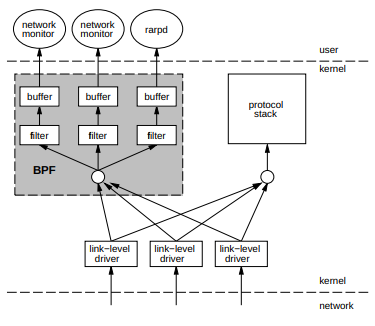
\includegraphics[width=\columnwidth]{./img/bpf_overview.png}
      \end{center}
      \caption{The overview of BPF architecture. It accelerates packet capture
                by performing filtering in the kernel space. \cite{mccanne1993bsd}}
      \label{img:bpf_old}
    \end{figure}
    
    また,eBPFがカバーする領域も拡大していった.ネットワークの文脈では,Linuxのネットワークスタックの様々なレイヤー,例えばUnix socket
    やネットワークデバイスなどを扱えるようになった.加えてeBPFプログラムはLinuxシステムのパフォーマンストレーシングやセキュリティ向上にも
    利用できるようになり,"BPF"という単語は本来の意味である"Berkeley Packet Filter"を失い独立した単語として使われるようになっていった.
    
    便宜上,v3.18における拡張以前のBPFをclassical BPF,あるいはcBPFと呼ぶことがある.
  
  \subsection{eBPFのアーキテクチャ}
    eBPFのアーキテクチャの概要を\Fref{img:ebpf-system}に示す.以下,\Fref{img:ebpf-system}を参照しながら重要な
    処理フローについて説明する.
    \begin{figure}[tp]
      \begin{center}
        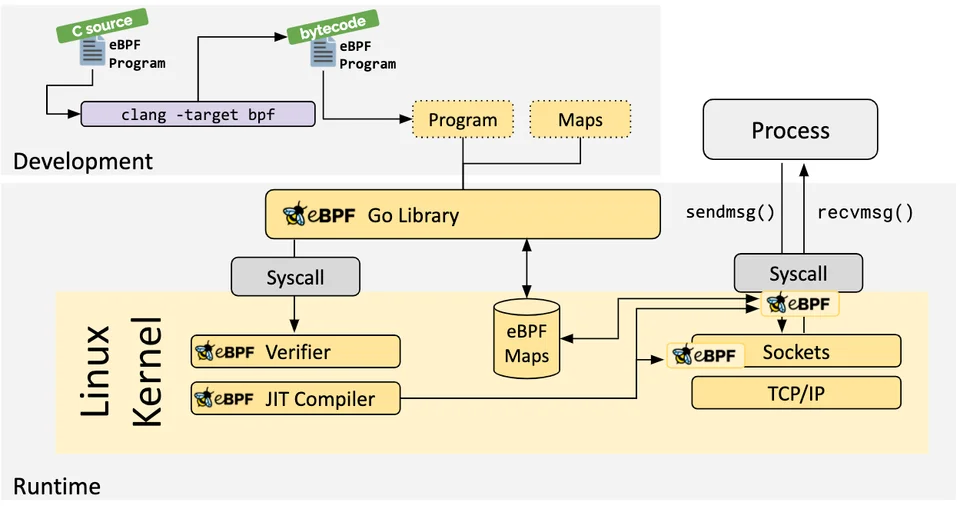
\includegraphics[width=\columnwidth]{./img/ebpf_system.png}
      \end{center}
      \caption{The overview of eBPF architecture. This figure shows how eBPF programs are compiled, verified, and executed.
      \cite{WhatiseB29:online}}
      \label{img:ebpf-system}
    \end{figure}

    \subsubsection{Event-Driven Architecture}
    eBPFはevent-drivenである.カーネル内でのイベントにeBPFプログラムをフックし,
    イベントが発生したら所定の処理を行う,という仕組みである.
    eBPFプログラムは動的にロードまたは削除することが可能である.
    
    eBPFがフックできるイベントはカーネルのソースコード \footnote{\texttt{include/uapi/linux/bpf.h}} においてProgram Typeとして定義されている.
    Program Typeをイベントの種別ごとに分類すると,以下のようなものが挙げられる.
    \begin{itemize}
      \item XDP: ネットワークデバイスにパケットが到着したとき,カーネル空間にデータがコピーされる前にパケットを操作するためのイベント.
      \item tracing: カーネル関数の呼び出しやトレースポイントの通過を検知するためのイベント.
      \item LSM: Linux Security Moduleを利用してセキュリティポリシーを適用するためのイベント.
    \end{itemize}
    
    このようなイベントが発生したとき,eBPFプログラムはProgram Typeに応じた処理を実行する.
    例えばXDPのイベントにフックされているプログラムがパケットをacceptするかdropするかを判断する,といった
    処理が可能である.
    
    \subsubsection{eBPF Verifier}
    eBPF verifierはバイトコードに変換されたeBPFプログラムを入力とし,そのプログラムがカーネル上で安全に
    実行できることを検証するプログラムである.バイトコードは\texttt{bpf()}システムコールで
    カーネル上にロードされる (\Fref{img:ebpf-system}の"Syscall") が,verifierによる検証を
    通過しない限りプログラムは実行されない.
    具体的には,メモリアクセス違反を起こさないことやプログラムが正常に終了すること,
    不必要なprivilegeがプログラムに与えられていないことなどが確認されている.
    
    このように,eBPF verifierはeBPFプログラムに制約を課すことで安全性を高めている.
    verifierがeBPFにおいて重要な意味を持つことから,verifierのロジックを数学的に検証する
    研究 \cite{vishwanathan2023verifying}も行われている.
    
    \subsubsection{JITコンパイル}
    verifierを通過したeBPFバイトコードはJITコンパイラによってターゲットのCPU上で直接動作する機械語に変換される.
    これにより実行速度が最適化され,ソースコードから直接コンパイルされたカーネルおよびカーネルモジュールと同程度効率的に
    動作する.
